
% Due thursday

\documentclass{article}

\usepackage[utf8]{inputenc}

\usepackage{amsmath, bm}
\usepackage{graphicx}
\usepackage{amssymb}
\usepackage{float}
\usepackage{caption}
\usepackage{subcaption}
\usepackage{hyperref}
\usepackage{tikz}
\usepackage{layout}

\usepackage[margin=1in]{geometry}
\usepackage{listings}
\usepackage{xcolor}
\usepackage{color, colortbl}
\usepackage{textgreek}
\usepackage{mathrsfs}
\usepackage{savetrees}


\setlength{\parskip}{\baselineskip}%
\setlength{\parindent}{0pt}%
\linespread{0.9}


\definecolor{codegreen}{rgb}{0,0.6,0}
\definecolor{codegray}{rgb}{0.5,0.5,0.5}
\definecolor{codepurple}{rgb}{0.58,0,0.82}
\definecolor{backcolour}{rgb}{0.95,0.95,0.92}

\lstdefinestyle{mystyle}{
    backgroundcolor=\color{backcolour},   
    commentstyle=\color{codegreen},
    keywordstyle=\color{magenta},
    numberstyle=\tiny\color{codegray},
    stringstyle=\color{codepurple},
    basicstyle=\ttfamily\footnotesize,
    breakatwhitespace=false,         
    breaklines=true,                 
    captionpos=b,                    
    keepspaces=true,                 
    numbers=left,                    
    numbersep=5pt,                  
    showspaces=false,                
    showstringspaces=false,
    showtabs=false,                  
    tabsize=2
}

\lstset{style=mystyle}



\begin{document}

\title{GA3: Heat Exchanger Performance Report}
\author{lwp26 - Group E}
\date{May 2024}
\maketitle 

\section{Introduction}

\section{Uncertainty Analysis}

\begin{equation}
    \dot{Q} = f(L_\text{tube}, Y, B, T_{1in}, T_{2in}) = f(x_1, x_2, \ldots, x_N)
\end{equation}

The relative uncertainty of $\dot{Q}$ due to variable $i$ is found numerically by a central difference method:

\begin{equation}
    u_i(\dot{Q}) \approx \frac{ \left| \dot{Q}(x_i + \delta x_i) - \dot{Q}(x_i - \delta x_i) \right|}{2\dot{Q}(x_i)} \label{eq:central_difference}
\end{equation}

An initial test was performed to determine the sensitivity of $\dot{Q}$ to baffle spacing, pitch and length.
The absolute uncertainty in baffle spacing, pitch and length is taken to be 1mm.
This represents a high relative uncertainty in the pitch due to the empirical method used in the software.
The relative uncertainty in calculated $\dot{Q}$ was found to be 0.00546\%, 0.58286\% and 0.11430\% for baffle spacing, pitch and length respectively.
This shows that an uncertainty in baffle spacing has negligible effect and is not considered in further analysis.
For all 2024 designs the number of tubes and baffles are equal across cross sections.

\subsection{Uncertainty of Inputs}

To perform further uncertainty analysis the uncertainty in input variables must be determined.
For length the uncertainty can be estimated from CAD drawings and manufacturing processes.
The uncertainty in the pitch is harder to determine.

Given that the CAD drawings are available, it makes sense to define a true average pitch and compare this to the calculated pitch to determine the uncertainty.
The true average pitch is defined as the average edge length of a network spanning a given hot section.
For all designs in 2024 the hot sections are circularly symmetric and so the average pitch is the same for all hot sections.
The absolute uncertainty in the pitch is then taken to be the maximum difference between the calculated and true average pitch.

\begin{minipage}[t]{0.29\textwidth}
    \centering
    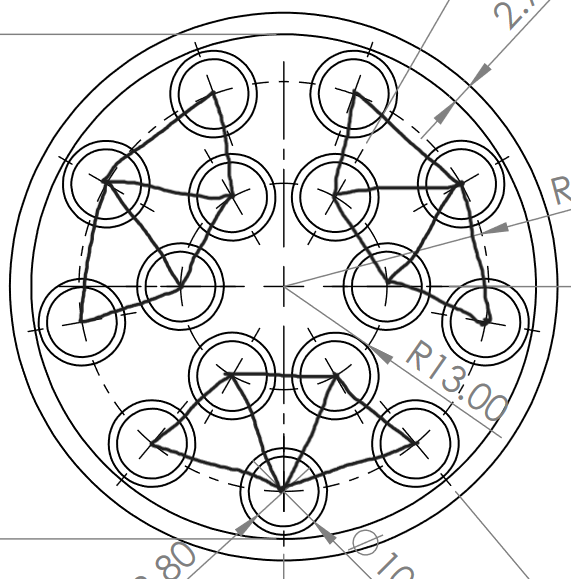
\includegraphics[width=0.8\textwidth]{tube_network.png}
    \captionof{figure}{Three tube networks in our heat exchanger design}
    \label{fig:tube_network}
\end{minipage}
\begin{minipage}[t]{0.69\textwidth}
    \centering
    \begin{tabular}{|c|c|c|}
        \hline
        Design & Calculated Pitch (mm) & True Average Pitch (mm) \\
        \hline
        A & 16.33 & 12.00 \\
        B & 16.33 & 15.41 \\
        C & 16.33 & 14.67 \\
        D & 15.21 & 12.00 \\
        E & 14.49 & 15.13 \\
        \hline
    \end{tabular}
    \captionof{table}{Pitch Comparison}
    \label{tab:pitch_comparison}
\end{minipage}

\subsection{Uncertainty of Outputs}
Corrections from available experimental data were applied to the pressure calculations to improve the accuracy Kerns method.
The uncertainty in mass flow from these corrections is not considered in this short report.
A correction was also applied to the final $\dot{Q}$ value as it had a strong correlation coefficient.
Uncertainty in the uncorrected $\dot{Q}$ was estimated for each variable by the same central difference method in equation \ref{eq:central_difference}.
These values are shown for each design in the table \ref{tab:uncorrected_uncertainty} below, along with the overall propagated uncertainty.

\begin{table}[h!]
    \centering
    \begin{tabular}{c|cccccc}
        \hline
        Group & $u_Y(\dot{Q})$ & $u_L(\dot{Q})$ & $u_{T_\text{1in}}(\dot{Q})$ & $u_{T_\text{2in}}(\dot{Q})$ & $u_\text{unc}(\dot{Q})$ \\
         & (\%) & (\%) & (\%) & (\%) & (\%) \\
        \hline
        A & 2.38 & 0.119 & 1.35 & 1.35 & 3.06 \\
        B & 2.31 & 0.127 & 1.32 & 1.32 & 2.97 \\
        C & 2.44 & 0.117 & 1.37 & 1.37 & 3.11 \\
        D & 3.17 & 0.132 & 1.32 & 1.32 & 3.68 \\
        E & 3.86 & 0.137 & 1.37 & 1.37 & 4.32 \\
        \hline
    \end{tabular}
    \caption{Relative uncertainty components of each groups design to each variable, and the uncertainty in uncorrected $\dot{Q}$ due to all variables.}
    \label{tab:uncorrected_uncertainty}
\end{table}

The correction applied to $\dot{Q}$ was based on a limited set of 2022 and 2023 data.
The uncertainty in the slope and intercept coefficients for this correction was estimated using a t-distribution with a 90\% confidence level.
This is displayed with the uncorrected uncertainty below in figure \ref{fig:uncertainty_regions}.

\begin{figure}[H]
    \centering
    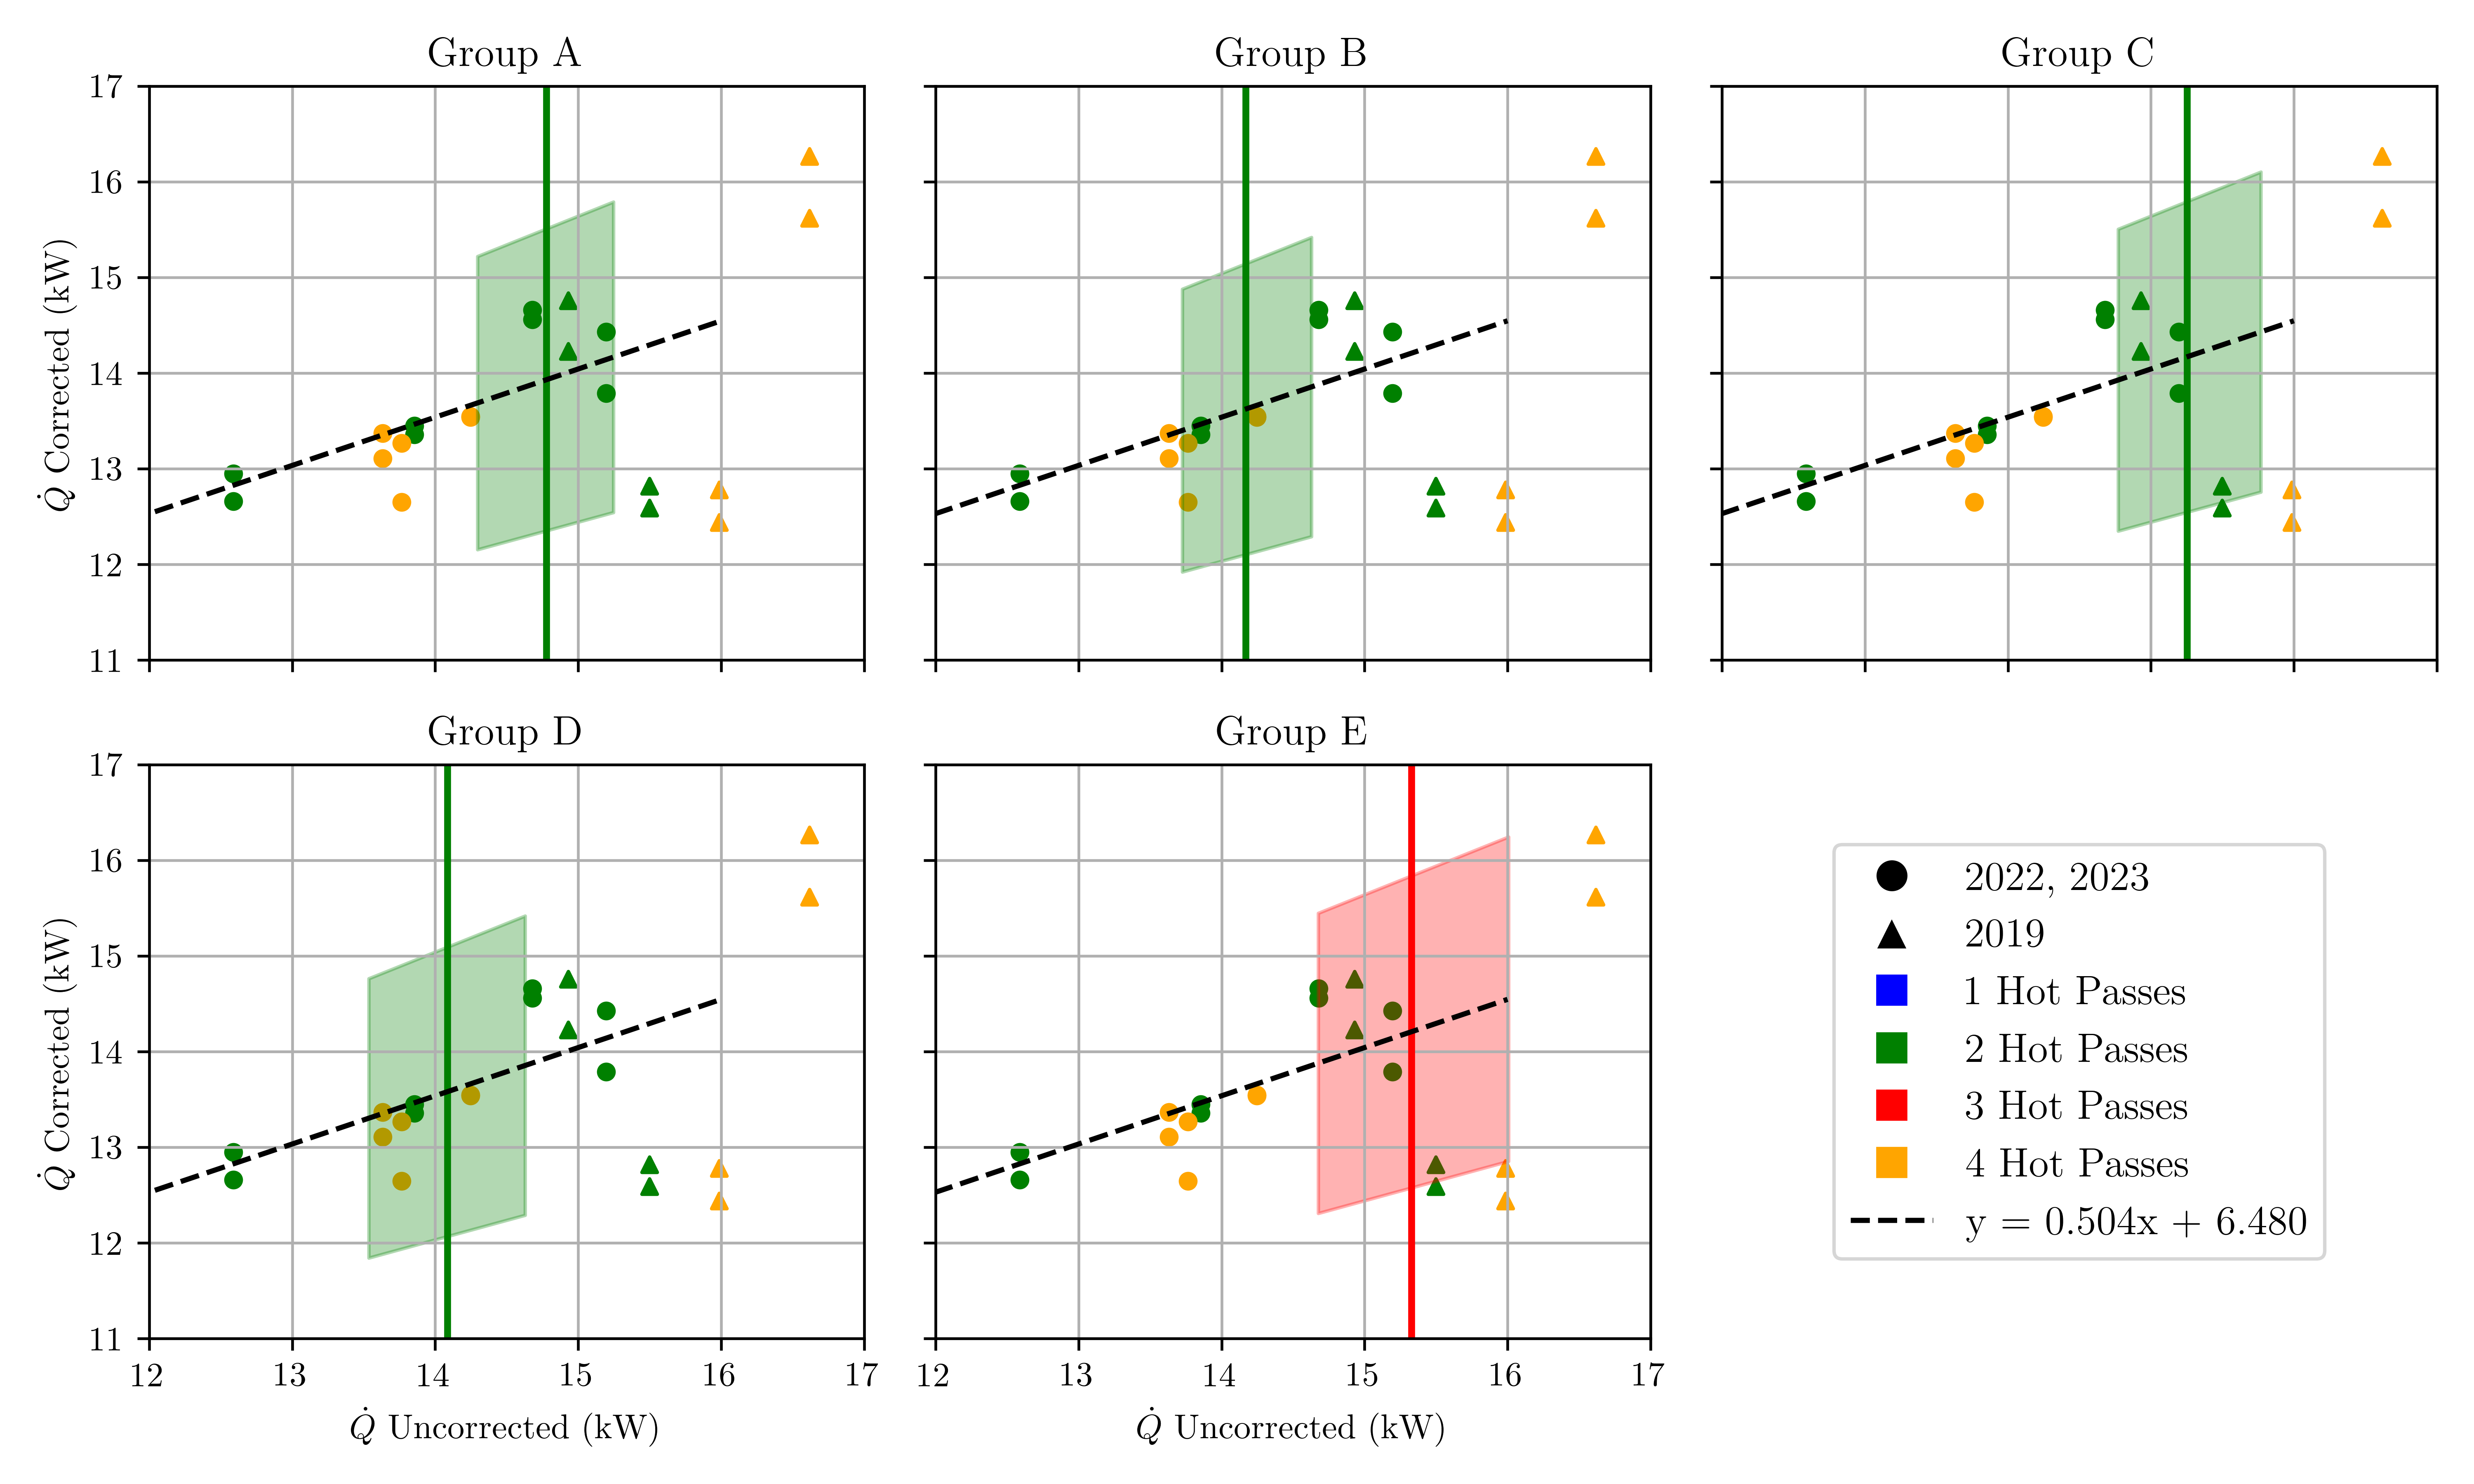
\includegraphics[width=0.99\textwidth]{Qdot_uncertainty_bands.png}
    \caption{$\dot{Q}$ Uncertainty Regions for 2024 Designs given uncorrected \ref{tab:uncorrected_uncertainty}}
    \label{fig:uncertainty_regions}
\end{figure}

\section{Performance Degradation}

Fouling is a common issue in heat exchangers, leading to a reduction in heat transfer.
This can be due to a variety of mechanisms depending on the fluid, geometry and operating conditions.
For feedwater heaters the most common fouling mechanisms are
This is often modelled by an empirical fouling factor, which acts as additional thermal resistance \cite{HeatTransfer}.

\subsection{Performance Comparison}


\begin{figure}[H]
    \centering
    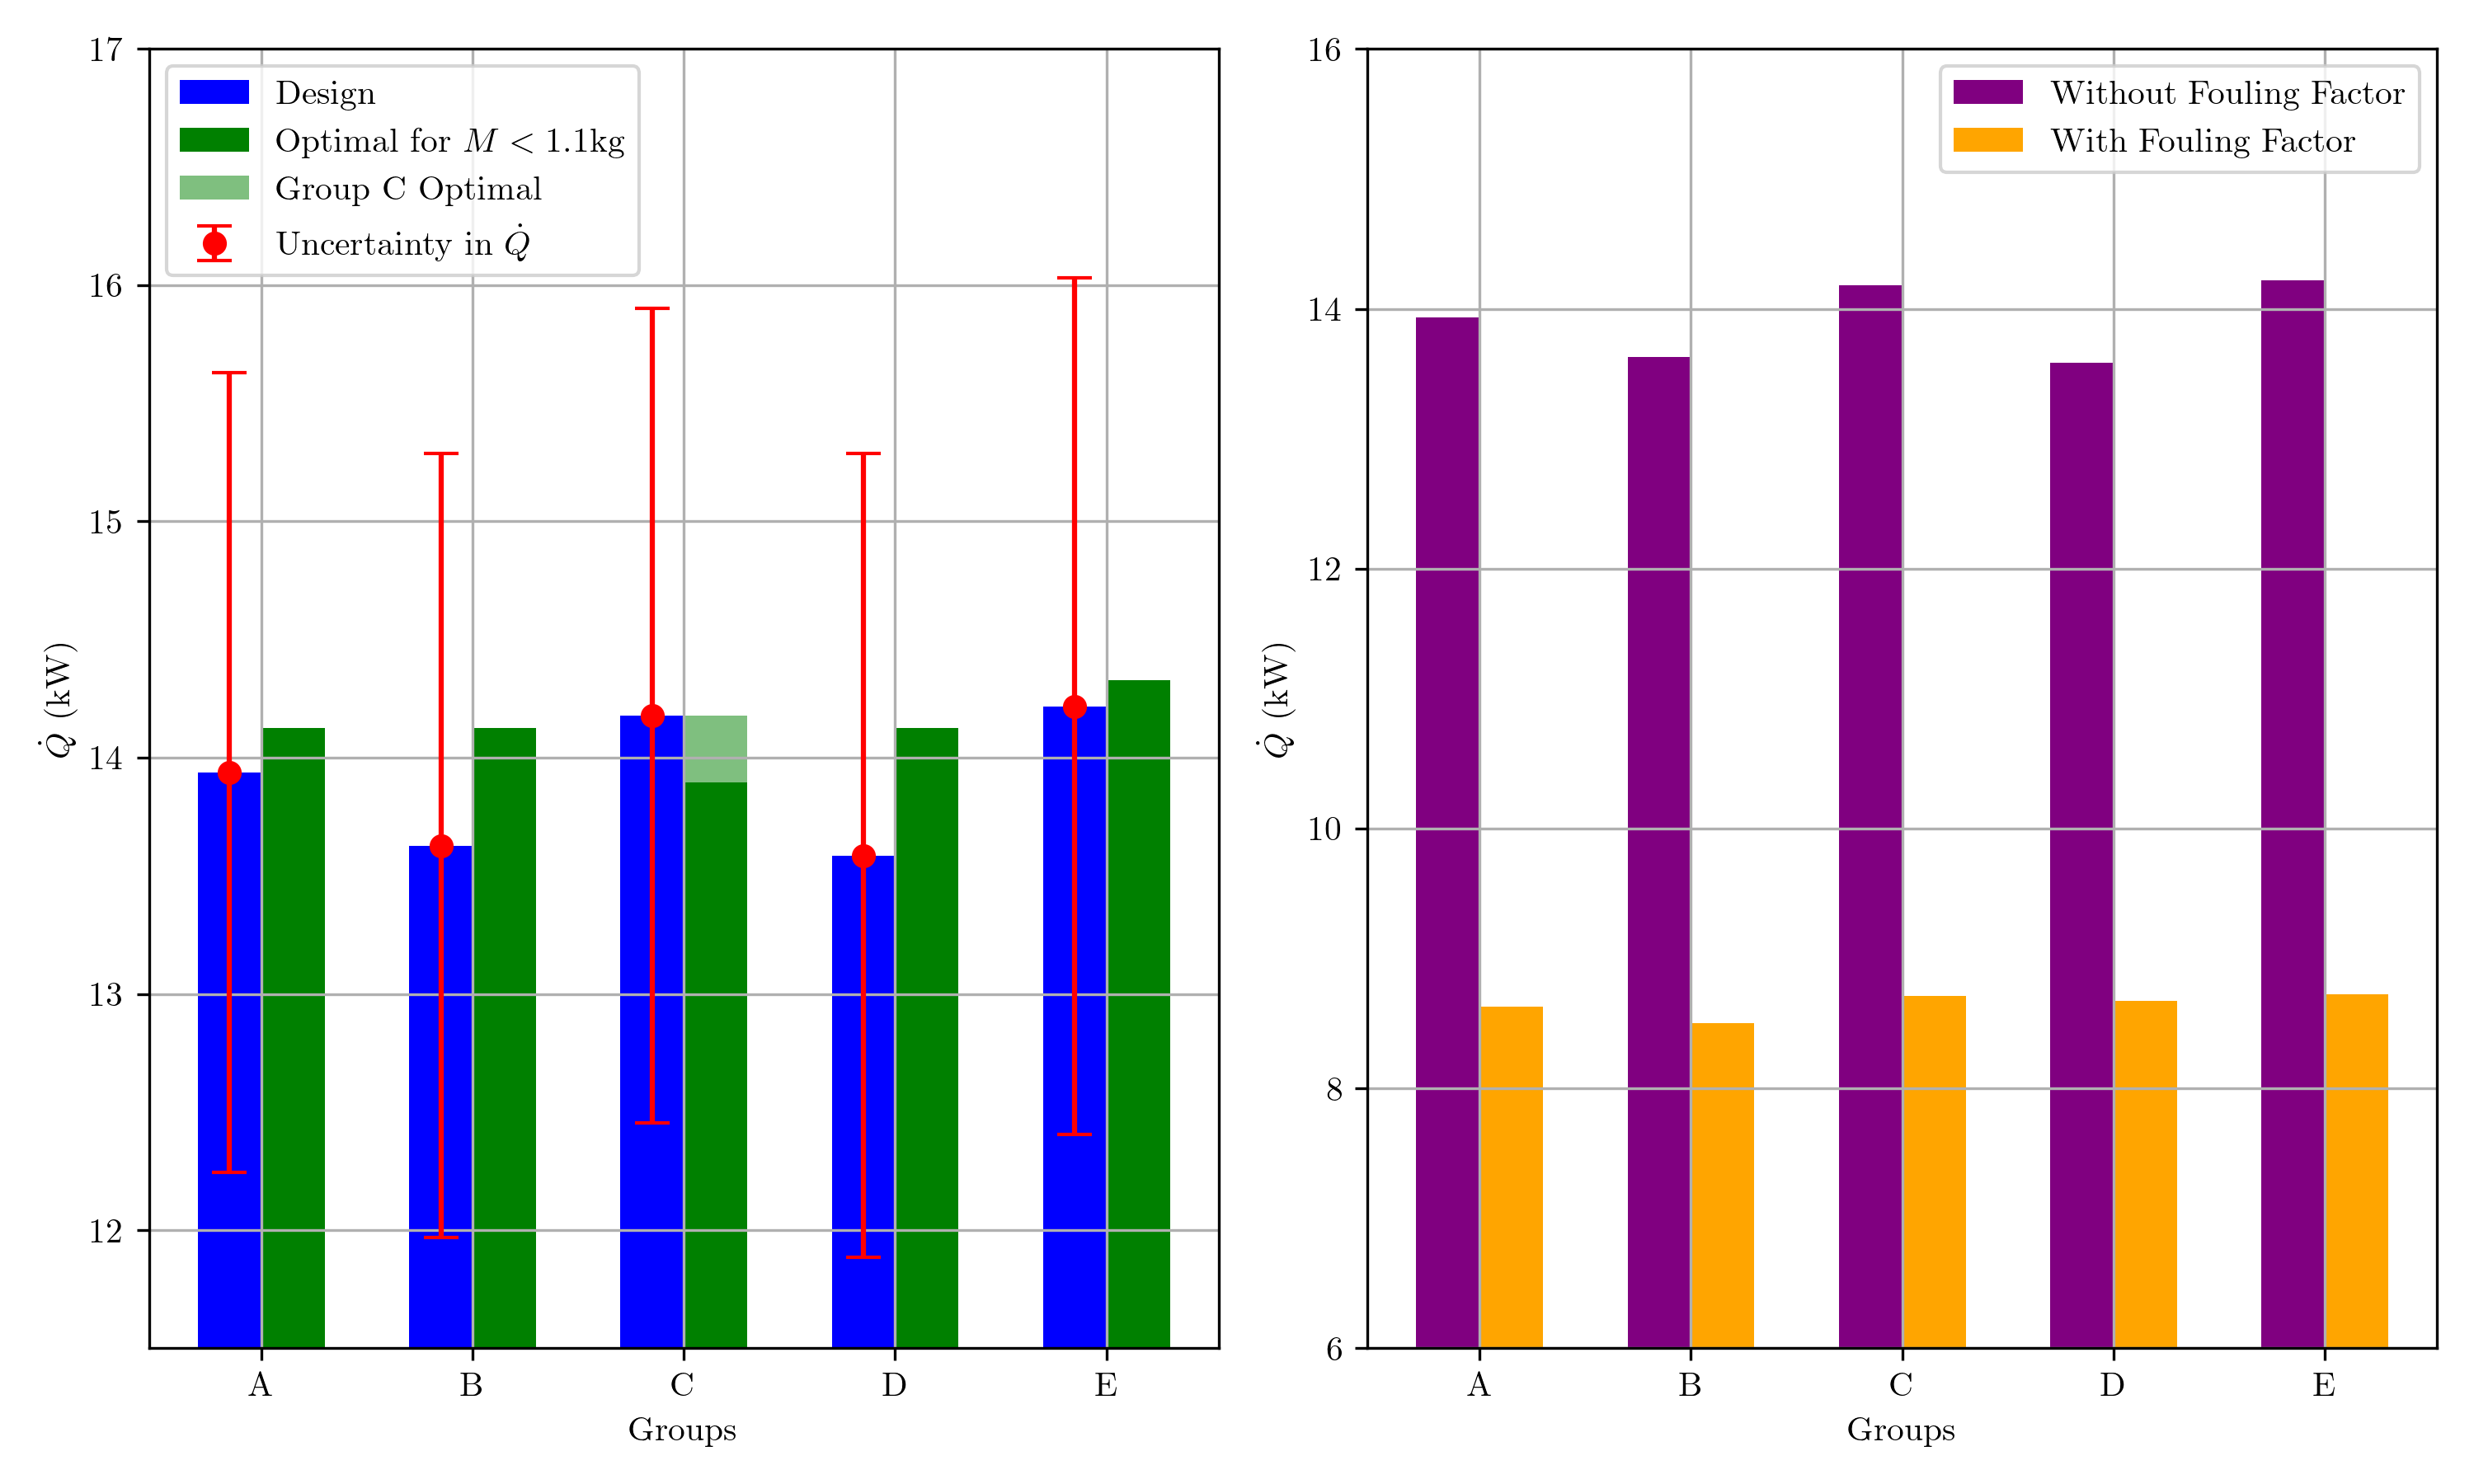
\includegraphics[width=0.8\textwidth]{2024comparison.png}
    \caption{2024 Performance Comparison}
    \label{fig:2024_performance}
\end{figure}

\begin{thebibliography}{9}

    %Endres, SC, Sandrock, C, Focke, WW (2018) “A simplicial homology algorithm for lipschitz optimisation”, Journal of Global Optimization.
    
      \bibitem{handout}
      J. V. Taylor and J. C. Massey
      \emph{GA3 Heat Exchanger Handout}
      University of Cambridge,
      2024.
    
      \bibitem{HeatTransfer}
      Holman J. P.
      \emph{Heat Transfer. 10th ed.}
      McGraw-Hill,
      2010.

      \bibitem{fouling}
      M. Ratel, Y. Kapoor, Z. Anxionnaz-Minvielle, L Seminel, B. Vinet
      \emph{INVESTIGATON OF FOULING RATES IN A HEAT EXCHANGER USING AN INNOVATIVE FOULING RIG}
      International Conference on Heat Exchanger Fouling and Cleaning
      2013

\end{thebibliography}


\end{document}